
%%%%%%%%%%%%%%%%%%%%%%%%%%%%%%%%%%%%%%%%%
% Short Sectioned Assignment
% LaTeX Template
% Version 1.0 (5/5/12)
%
% This template has been downloaded from:
% http://www.LaTeXTemplates.com
%
% Original author:
% Frits Wenneker (http://www.howtotex.com)
%
% License:
% CC BY-NC-SA 3.0 (http://creativecommons.org/licenses/by-nc-sa/3.0/)
%
%%%%%%%%%%%%%%%%%%%%%%%%%%%%%%%%%%%%%%%%%

%----------------------------------------------------------------------------------------
%	PACKAGES AND OTHER DOCUMENT CONFIGURATIONS
%----------------------------------------------------------------------------------------

\documentclass[paper=a4, fontsize=11pt]{scrartcl} % A4 paper and 11pt font size

\usepackage[T1]{fontenc} % Use 8-bit encoding that has 256 glyphs
\usepackage{fourier} % Use the Adobe Utopia font for the document - comment this line to return to the LaTeX default
\usepackage[english]{babel} % English language/hyphenation
\usepackage{amsmath,amsfonts,amsthm} % Math packages
\usepackage{gensymb}
\usepackage{chemmacros}
\usepackage{sectsty} % Allows customizing section commands
\usepackage{graphicx}
\allsectionsfont{\centering \normalfont\scshape} % Make all sections centered, the default font and small caps

\usepackage{fancyhdr} % Custom headers and footers
\pagestyle{fancyplain} % Makes all pages in the document conform to the custom headers and footers
\fancyhead{} % No page header - if you want one, create it in the same way as the footers below
\fancyfoot[L]{} % Empty left footer
\fancyfoot[C]{} % Empty center footer
\fancyfoot[R]{\thepage} % Page numbering for right footer
\renewcommand{\headrulewidth}{0pt} % Remove header underlines
\renewcommand{\footrulewidth}{0pt} % Remove footer underlines
\setlength{\headheight}{13.6pt} % Customize the height of the header

\numberwithin{equation}{section} % Number equations within sections (i.e. 1.1, 1.2, 2.1, 2.2 instead of 1, 2, 3, 4)
\numberwithin{figure}{section} % Number figures within sections (i.e. 1.1, 1.2, 2.1, 2.2 instead of 1, 2, 3, 4)
\numberwithin{table}{section} % Number tables within sections (i.e. 1.1, 1.2, 2.1, 2.2 instead of 1, 2, 3, 4)

\setlength\parindent{0pt} % Removes all indentation from paragraphs - comment this line for an assignment with lots of text

\graphicspath{
	{./Figures/}
}
%----------------------------------------------------------------------------------------
%	TITLE SECTION
%----------------------------------------------------------------------------------------

\newcommand{\horrule}[1]{\rule{\linewidth}{#1}} % Create horizontal rule command with 1 argument of height

\title{	
\normalfont \normalsize 
\textsc{Universit\"{a}t Basel} \\ [25pt] % Your university, school and/or department name(s)
\horrule{0.5pt} \\[0.2cm] % Thin top horizontal rule
\huge TissueCyte User Manual % The assignment title
\horrule{1.5pt}\\ % Thick bottom horizontal rule
}


\date{\normalsize\today} % Today's date or a custom date

\begin{document}

\maketitle % Print the title

This document was compiled at the University of Basel and describes our operating procedures for the TissueVision 1000 2-photon tomography system.


\section{Basic operating principle}
The system comprises a conventional 2-photon microscope with a motorized 3-axis stage and a custom vibrotome. 
The objective and blade are fixed, whilst the sample is moved beneath them. 
The sample is embedded in an agar block glued to a microscope slide which is magnetically attached to a steel plate at the bottom of a small water bath.
The water bath is attached to the $x$/$y$ stage mounted on a vertical jack. 
Thin slices are automatically cut from the face of the block and the block face imaged. 

\begin{figure}[h]
\centering
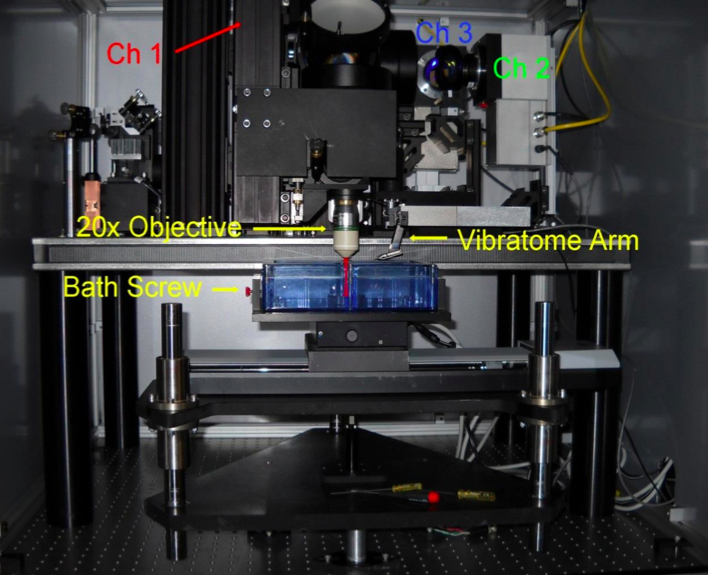
\includegraphics[width=0.45\textwidth,natwidth=708,natheight=575]{scopeImage.png}
\caption{Front view of the TissueCyte microscope.}
\label{fig:scope_front}
\end{figure}


\clearpage

\section{Warnings}
The system has few fail safe measures in the event of improper usage.
Follow these guidelines:
\begin{enumerate}
\item The collection light path is not enclosed and the sensitive PMTs can gather light from the room directly.
\textbf{Do not} expose the PMTs to room lights when they are powered. 
Always double-check (literally, double-check) that the doors are shut and the lights are off before applying power to the PMTs. 
\item Always move the sample gradually towards the objective in order to avoid them crashing together. 
The software has no working stop button (ignore the large button labeled `stop'. It doesn't do anything useful). 
We have added a hardware stop button which can be used in case of emergencies. 
Make sure you have been trained on how to use this, as when you press it you will need to restart the acquisition software. 
\item The objective is heavy and comes away suddenly when being unscrewed for cleaning. 
Always unscrew with one hand whilst supporting the objective with the other. 
If you're unsure, keep something soft underneath the objective whilst unscrewing.
\end{enumerate}


\section{Software list and acquisition PCs}
The system uses three computers: two for the acquisition machine and one to control the laser.
The acquisition machines machines are controlled via a single keyboard and mouse. 
The monitor for the `master' computer is on the left and that for the `slave' computer is on the right. 
The master acquires data from channel 1 and controls the hardware. 
The slave computer acquires data from channels 2 and 3. 
Data are streamed to a 40 TB QNAP NAS, which is \textit{not backed up}.
The laser control machine can be accessed from home via RDP and VPN, avoiding late night trips to work to turn off the laser.


\subsection{Useful points}
\begin{enumerate}
\item Should the acquisition software crash or otherwise lock up, close all of the windows (including the black terminal windows) and re-start the software.
Restarting the software means you have to again `reference' (zero) the $x$/$y$ stages.
\item Always ensure that the QNAP (`tvbuffer') is mounted on both the slave and the master computers. 
If it is not, the system will hang without explanation if you attempt to save data to it.
\item Every time you press the green `2D' button in Orchestrator tiffs are saved to:\\
\texttt{C:\textbackslash \textbackslash TissueVision\textbackslash MicroscopeData}  
\item If you issue a stage motion command that would take the stage out of bounds a small warning dialog is created. 
This message blocks further actions in Orchestrator, but appears below all other windows so you can't see it.
To proceed, you need to look for the message box on the taskbar, find window and click `OK.' 
\end{enumerate}

\section{Running a sample through the system}
Setting up a sample for imaging takes approximately an hour when all is working as expected. 
The phases of the process are as follows:

\begin{itemize}
\setlength\itemsep{0.01em}
\item Getting the sample onto the stage and attaching the blade.
\item Slicing through the block until the sample is exposed.
\item Finding the sample surface.
\item Checking that the system is cutting reliably at the desired section thickness. 
\item If applicable, ensuring the laser power settings are reasonable across depths. 
\item Determining the number tiles in $x$ and $y$ required to cover the sample. 
\item Identifying the start position for imaging and moving to this position. 
\end{itemize}


\subsection{Getting the sample into the scope}

\begin{itemize}
\item Turn on the laser via the SpecraPhysics GUI on the far right PC. 
The square green `laser pulsing' indicator should come on. 
\item If the PMT GUI is already is open, ensure the PMTs are switched off (Fig.~\ref{fig:pmt}).
\item The sample is glued to a slide and the slide magnetically attached to the sample bath. 
Fill the bath with 1,200~ml of PB. 
\item Transfer the sample bath to the stage and centre it in the holder.
Tighten the red retaining screw one eighth of a turn beyond the point at which it first contacts the bath. 
\item Add a new blade to the blade holder and tighten with the two screws behind the blade.
These screws should be snug but not over-tight. 
Tighten them alternately and gradually: if you over-tighten one screw first the blade can fall out. 
\item Attach the blade holder to the vibrotome. 
\end{itemize}

\begin{figure}[h]
\centering
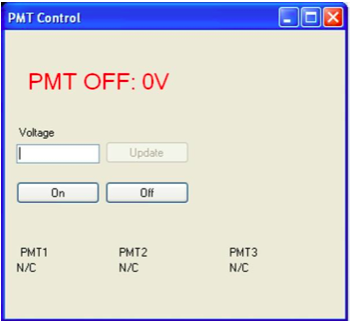
\includegraphics[width=0.3\textwidth,natwidth=354,natheight=324]{PMT_GUI.png}
\caption{The PMT GUI with the PMTs off.}
\label{fig:pmt}
\end{figure}

\clearpage

\subsection{Navigating down to the sample}
You will now navigate down to the surface of the agar block using the Orchestrator program on the Master acquisition PC.

\begin{itemize}
\item Open Orchestrator on the master computer. 
The icon is in the desktop. 
Open the client program on the slave computer (this is the green arrow on the desktop). 
In the first tab (Fig.~\ref{fig:serv_tab}) in Orchestrator click `connect all', `slave', and `reference stage.' 
If the slave connection worked, a new window will appear on the slave screen.

\item It is now time to raise the bath. 
Remember that it's possible to go too far and smash either the blade or the objective into the sample. 

\item It is definitely safe to raise the stage 15~mm. 
Type 15000 (all distance measurements are in microns) into the $z$-stage dialog box (third tab over, Fig.~\ref{fig:im_tab}) and press `up', as you are moving the sample \textit{upwards} with respect to the objective. 
Go and watch the stage move. 
Be ready with the hard-stop button box.

\item Once the motion has finished you'll know how much further you need to go. 
Move up gradually. 
The goal is to get the blade within about 1~mm of the sample in $x$ and very close to the surface height in $z$. 
This will yield a thin first cut.

\item Move the stage 20~mm \textit{to the left}. 
The sample should now be near the objective. 
Roughly center the sample under the objective and keep in mind roughly how far you've moved the sample.

\end{itemize}

\begin{figure}[h]
\centering
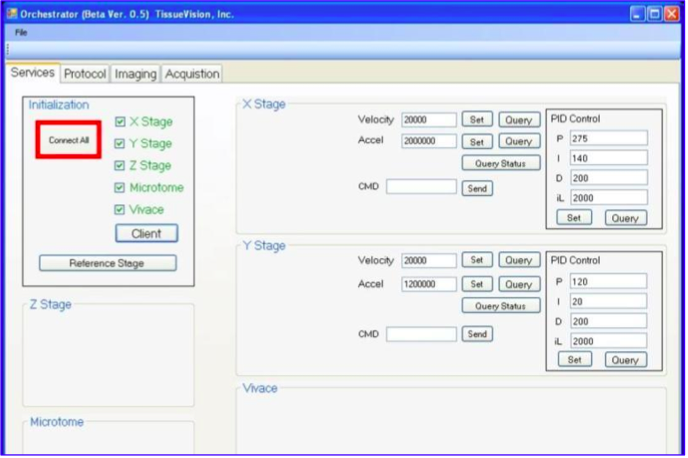
\includegraphics[width=0.8\textwidth,natwidth=688,natheight=548]{services_tab.png}
\caption{The services tab.}
\label{fig:serv_tab}
\end{figure}



\subsubsection{Exposing the surface of the sample}
You will now begin cutting in order to expose the surface of the sample. 
\textbf{Critical info}: following any change to parameter settings in the parameter tab (second tab, Fig.~\ref{fig:prot_tab}), you should press the `Update' button. 
If you fail to do this, your changes aren't implemented.

\begin{itemize}
\item At this stage you will begin to change parameters that ultimately will influence how you image. 
On the second tab in the top left you should load a suitable parameter file (the names are descriptive).

\begin{enumerate}
\item Load an existing parameter file most closely resembling what you're doing (you can tell by the names) and modify as needed.
\item You often will need to make minor changes to a file. 
Usually the number of depths. 
Make these and save you file as as `Last\_Protocol.xml' (just over-write the existing one). 
The acquisition software can crash or lock up during setup, so you'll save time if you can re-load your progress quickly.

\end{enumerate}
\item Provide a directory and name for your experiment. 
In the protocol tab, choose a save path. 
Each experiment should have its own directory.
This ensures Orchestrator doesn't over-write existing data and the analysis routines assume a single experiment per directory. 
\item Ensure you have a sensible sample ID in the protocol tab. 
If not Orchestrator comes up with unique junk-name ID.
Restrict yourself to alphanumeric characters and hyphens for the sample ID name and directory: it's safer.
\item You will now begin to cut. 
  Before doing so, you need to be familiar with what happens with the `slice' (3rd tab) is pressed:
 \begin{enumerate}
  \item The $z$-stage moves up by one section thickness. This value is defined in the section thickness box (2nd tab).
  \item The $x$-stage is moved rapidly to the right by $x~\mu m$, where $x$ is user-definable. How far it moves is determined by the 
  `Microtome Position' value. 
  \item The blade starts to vibrate.
  \item The $x$-stage moves slowly at the user defined cutting speed (`Sectioning Speed') for about 35~mm.
  \item The $x$-stage pauses for `Delay' period to ensure the section settles to the bottom. 
  \item The sample is returned to the pre-slice $x$/$y$ position. 
 \end{enumerate}
\item You want to set the fast motion value to a reasonable number. e.g. say you moved 20~mm from the 
blade to the objective and the sample was more or less in the right place. You could safely set the fast motion value to 18~mm.

\item Set the section thickness to about $100~\mu m$ (Protocol tab) and press the `Slice' button (Imaging tab) and watch it cut. 

\item Once you're cutting in the block and things seem good, you need cut until you're near or in the sample. 
Keep the sectioning speed below about $0.75~mm/s$ and you'll be able to cut thick slices (even $1,000~\mu m$ or so). 

\item As you approach the sample surface, you should begin to decrease the section thickness and slow the sectioning speed. 
It seems that gradually approaching the section thickness is more likely to produce good results. 
Once you have reached the section thickness you are aiming for, ensure the slices are coming off cleanly without shredding.
If the sectioning doesn't \textit{look} clean to the eye, then you will get appalling results if you attempt to image. 
Sections of $80~\mu m$ and thicker should work well at a speed of $0.5~mm/s$. 
For $40~\mu m$ or $50~\mu m$ sections you may need to drop down to speeds of about $0.35~mm/s$.
\end{itemize}




\begin{figure}[h]
\centering
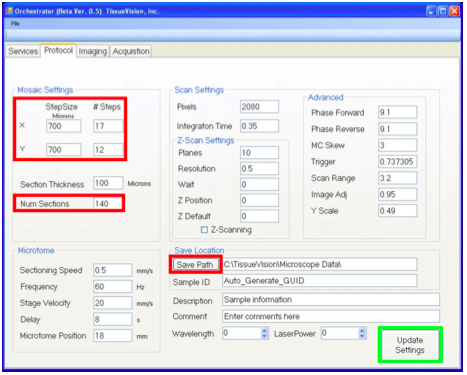
\includegraphics[width=0.8\textwidth,natwidth=467,natheight=375]{protocol_tab.png}
\caption{The protocol tab.}
\label{fig:prot_tab}
\end{figure}

\begin{figure}[h]
\centering
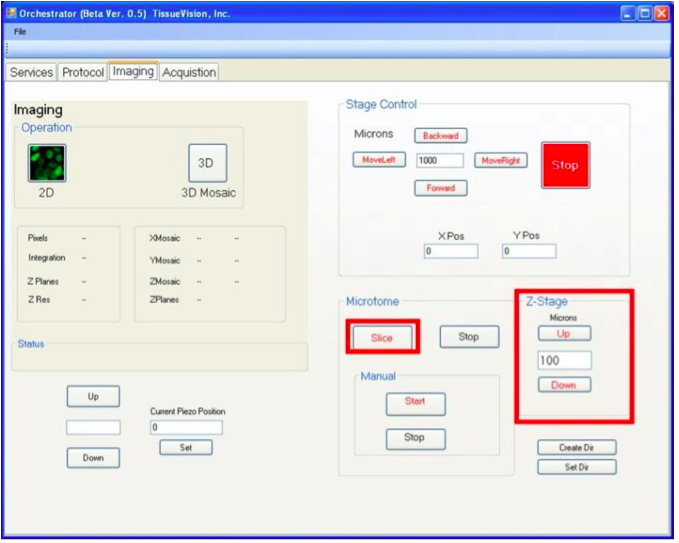
\includegraphics[width=0.8\textwidth,natwidth=679,natheight=543]{imaging_tab.png}
\caption{The imaging tab.}
\label{fig:im_tab}
\end{figure}
\clearpage

\subsection{Finding the sample surface}
The goal of this step is to locate the surface of the brain and ensure that the cutting plane and imaging planes are very 
near (within about $200~\mu m$). This is one of the more dangerous steps in the process as careless use of the lights can damage the 
PMTs and it's possible to push on the PIFOC, damaging it. Take your time here. 

\begin{itemize}
\item Open the laser shutter on the Spectra-physics GUI and tune the laser to 800~nm.
\item Go to the third tab in Orchestrator. Where it says says laser power, there are two numbers `V1' and `V2'. These are
the voltage values fed to the Liquid Crystal Variable Retarder (LCVR) \footnote{A variable half-wave plate, altering the angle 
of polarisation of light into a beam-splitter cube and thereby altering intensity}. Above these are a dialog box that sets the
laser power:
\begin{enumerate}
\item Closed: minimum power constantly.
\item Open: laser is constantly `on' at the power level specified.
\item Automatic: laser is only on during scanning. 
\end{enumerate} 

\item The `V1' value is that which the LCVR is at when the laser is off. The `V2' value is that which the LCVR is at when
the laser is on. One startup these values are inverted (don't ask why, they just are). Set V1 to 20 and set V2 to 3.2V. 
Press `state'.

\item Set the shutter state to `open' and press `state'. You should now see light from the beam exiting the objective. 
Don't proceed until you get this.

\item Use the $x$/$y$ controls to position the beam such that it hits the top surface of the sample. 

\item Set the shutter state to `close', press `state', then set it to `automatic.' This shuts off the laser power to the sample 
and ensures power is only delivered during imaging. 

\item Now you are ready to attempt imaging the surface.
 \textbf{Turn off the lights}. 
 Close and latch the enclosure (right door first).

\item Set the gain to 700~V in the PMT GUI. Green lettering indicates the PMTs are on! 

\item Press the green `2-D' scan button on the third tab of orchestrator. If all goes well, you will see two image windows appear 
on the slave screen and one on the master computer screen. If you are lucky you will see your sample. If not, you'll have to find it. 
We will  proceed assuming your sample was not visible. 

\item First of all you will want to set the range of values on the image windows to something reasonable. By default they auto-scale. 
Using the pull-down menu set each channel to `manual' and set the maximum value to about 1000. You don't need to press return after
 entering this value. 
 The windows aren't re-sizable.

\item If you did the sample is not visible, ensure the objective is over the brain, the PMTs are powered, the laser is modelocked, and the shutter is set to `Automatic.'
If the sample is still not visible, the likely you are at the wrong depth. 
Try moving the PIFOC over its $400~\mu m$ range with the rotary knob on the PIFOC control box. 

\item If you still can't find the surface, then you will need move the objective. 
Set the PIFOC to about $200~\mu m$ and begin hunting the surface with the objective depth adjustment knob. 
If you don't know how to do this read the objective height adjustment protocol (Section~\ref{objheight}, p.~\pageref{objheight}). 

\item Once you have found the surface of the brain and it is located roughly around $200~\mu m$ then you're ready to move on to checking the cutting reliability. 

\item \textbf{Remember} you want to be at the \textit{surface} of the sample, not somewhere in the middle. 
When you see the surface you will likely also notice the striations left by the blade cutting. 
You should certainly be able to see the sample vanish if you move the objective up a few microns ($5~\mu m$ to $10~\mu m$) from the surface. 
If you can not see this then you aren't at the surface. 
\end{itemize}



\subsection{Checking the cutting reliability}
\begin{itemize}
\item Find the surface by moving the PIFOC up and down. 
\item Cut at the speed and thickness you intend to use.
\item Image. Where is the surface? Move the PIFOC up and down and note the depth.  
\item If the surface has moved only about $5~\mu m$ to $10~\mu m$, that is fine. 
If not, try cutting again. 
You may find you need a few before it stabilises. 

\item If the surface is not stabilising the system may be in a cycle where it alternately cuts then fails to cut (or partially cuts). 
When this happens you may see fluctuations in surface height of well above $50~\mu m$ from cut to cut.
The system will not settle unless you try re-cutting thicker then going back to thinner sections, cutting slowly, or changing blades.
\item Do not proceed until you have the surface height deviation from cut to cut is no more than about $15~\mu m$. 
\item Once you're happy with the reliability, move the PIFOC about $35~\mu m$ down and take an image. 
This will be your imaging depth (or the top imaging plane in the event that you are taking optical sections). 
\end{itemize}

\clearpage

\subsection{Setting the power}
Take an image and check the brightness. If imaging a brain, don't use white matter as a test area since it's strongly scattering. 
You are aiming to achieve a reasonable signal in your channel(s) of interest with the channel's maximum pixel value set 
between about 3,000 and 4,000. 
Do not expect to use the full 16 bit dynamic range. 
To begin with, you're probably looking at auto-fluorescence right now so your actual signal will be much brighter. 
In addition, very bright signals (e.g. the region around a cortical injection) can easily be bright enough to cause the amplifiers to ring.
You will figure out with experience how much laser power is right for your sample. 
To help with this, we have positioned a photodiode behind one of the mirrors in the light path. 
We have created a look up table that links the value produced by the photodiode with a power reading at the objective. 




\subsection{Optical sections}
Say you are taking $100~\mu m$ cuts. 
To sample the tissue with a resolution of $50~\mu m$ you'd take two optical sections spaced $50~\mu m$ apart. 
For $25~\mu m$ resolution you'd take 4 optical sections spaced $25~\mu m$ apart. etc. 
To take optical sections set the required number of planes in the Protocol tab (`Planes', Fig.~\ref{fig:prot_tab}). 
You also need to tell the software the distance between the planes. 
You do this in the `Resolution' box, below the `Planes' box. 
The value you enter should be \textbf{half} the distance between optical sections. 
e.g. if you want to take optical sections every $25~\mu m$, you should enter 12.5 into the box.
Once done, make sure the two z-scanning check boxes are both ticked. 

Finally, you want to ensure that you get reasonable illumination as you go deeper. 
The system is able to ramp up the laser power with depth. 
As you go deeper, the PSF will degrade due to aberrations induced by the tissue and you will lose emitted photons due to scattering.
Thus the deeper depths will never look as good as the upper ones.
Nonetheless, you can move the PIFOC down to your lowest depth, increase the power value and take an image to confirm what intensity you should be imaging at. 
To tell the system to ramp power do the following:
\begin{itemize}
\item There is a directory on the desktop containing files with the extension `.csv'. 
These are just lists of power values, one per optical section. 
These files are named so as to indicate the wavelength and number of optical sections. 
\item Once you have the file, drag a copy over to the experiment directory. 
You now have a log of what you used for this sample. 
\item Go to the protocol tab. There is browse button near the middle of the screen to allow you to select your z-illumination file. Go here and select it. 
\item Make sure that you set the power in the Imaging tab to the power the system should be at for the first depth. 
\end{itemize}


\clearpage


\subsection{Setting up the acquisition}
You will need to determine the size of your sample in $x$ and $y$ as well as the positions of the front and left edges. 
If you are working with an adult mouse brain, you simply need to find the front and left edges since the size of the brain itself is known (usually 16 by 10 tiles). 
Use the laser to find the edges. 
Position the laser at the front/left position to start. 
For other samples, there is a spreadsheet to help you with calculating the number of tiles. 
It is easiest to be shown this procedure by an experienced user.



\subsection{Acquiring data}
\label{acqData}
At this point everything should be set up, but double-check it: objective position, laser wavelength, shutter set to `Automatic', etc.
Check the protocol file is saved as (e.g. as `Last\_Protocol.xml') and that you have written down the $x$/$y$ start location in case you need to re-start the acquisition.
If all looks good, press the `3-D' button to acquire data. 
After a short pause, the syste will start acquiring data.
Data acquisition can not be paused. 


\subsection{Re-starting the acquisition}
Protocol for restarting an acquisition that has failed in some way:
\begin{enumerate}
\item Close all the Orchestrator and Vivace windows on both machines. 
\item Re-open them all. Load the protocol XML file. Use the same sample name as before.
\item Move the stage the front-left start position (it's a good habit to note this down when you set up the sample).
\item Save the new acquisition in a new directory. 
\item You are going to re-image the section at which the acquisition failed.
Ammend the number of sections to image to be the difference between the original total number and the number that have already been acquired. 
Then you want to start the section numbering (also a box in the Protocol tab) at the number at which it failed. 
e.g. if it failed on section 135 then sect the start section number to 135. 
Do all the rest of your set up as before (laser power, etc) and start the acquisition
\end{enumerate}






\subsection{Shutdown}
\begin{itemize}

\item To stop scanning you simply close all the acquisition wondows (including the terminal windows).
The software will report it has crashed. This is normal.

\item Turn off the laser. 
You can do this from home if the machine has RDP access.

\item Before opening the enclosure, ensure the PMTs are switched off and the PMT GUI is closed.

\item Lower the stage about $35~mm$. 
Remove the blade holder and the blade. 
The blade is a safety hazard, do not leave it attached.

\item Wash the objective with distilled water, allowing the water to be collected by the sample bath. 
Remove the bath. 
Carefully clean the objective with lens tissue: it can get grimy over time.

\end{itemize}



\section{Objective Height Adjustment}
\label{objheight}
If you change to a new blade type or adjust the blade holder you will need to adjust the objective height. 
You will know you need to do this if you are over your sample and everything is set up correctly but you can not find the surface of the sample (or even see the sample at all) when manually seeking with the PIFOC. 
If you don't have enough range with the PIFOC for optical sectioning, you will also need to adjust the objective height. 

The goal of the objective height adjustment is to get the image plane at roughly the same level as the sample surface. 
In other words, the image plane and the blade tip need to be at the same level. 
Since the blade is fixed, your only option is to move the objective.

The objective is screwed into the PIFOC, which itself is clamped into a metal plate (see Fig.~\ref{fig:objHeight}). 
The metal plate is attached to a translation stage that moves the whole arrangement up and down. 
Screwing \textit{in} the adjustment bolt will push down the translation stage and \textit{lower} the objective. 
\textit{Unscrewing} the adjustment bolt allows the translation stage to be raised. Note that the translation 
stage is not sprung and must be push upwards by hand after the adjustment screw is turned. 
There is a lock bolt on the stage. 
Because it's hard to reach and because the stage is so stiff, the lock bolt is usually left loose. 
To change the objective height do the following:

\begin{figure}[h]
\centering
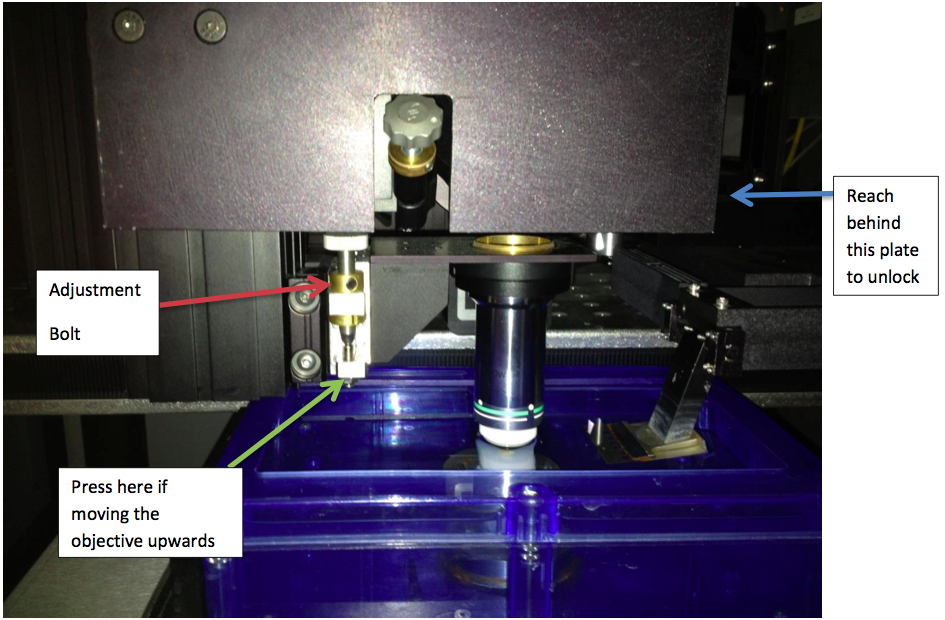
\includegraphics[width=0.8\textwidth,natwidth=945,natheight=620]{objHeight.png}
\caption{Objective height adjustment}
\label{fig:objHeight}
\end{figure}

\begin{enumerate}
\item Check whether the objective translation stage lock bolt needs loosening (unlikely):

\begin{itemize}
\item The screw locking the objective in place is located behind the objective. To
turn it, reach to the right of the objective between the vibrotome and the objective holder. 
The screw is located directly opposite from the adjustment bolt.

\item Avoid touching the primary dichroic or any of the large collection lenses.

\item Gently turn the screw until it loose. Do not remove it, just a quarter counter clockwise turn is sufficient.
\end{itemize}

\item Turn off the room lights. It's OK to leave the doors of the enclosure open in order to alternate between moving the objective and imaging.
It helps to do this with two people. 

\item Translate the objective using the adjustment bolt. Rotate the bolt to move the objective up or down, if you moved up, be sure to press beneath the bolt on the stage, and verify that the stage engaged the bolt after you moved it.
\begin{itemize}
\item If you know which way to move (e.g. move down if you put in a longer blade) then move that way.
\item If you don't know, then it's likely easiest to move down until you're near the sample then move up.
\item If moving up, remember that you need to turn the screw then push up the translation stage. 
Be sure that you do not push upwards on either the objective or the PIFOC. 
You may damage the PIFOC. 
If you don't know what the PIFOC looks like, then get help.

\item Do \textbf{not} seek up and down with the z-stage controls on the software. 
If you do this you will change the cutting depth on your next slice and you will become very confused about where the surface is. 

\end{itemize}

\item Take an image. 

\item Repeat until the sample surface is visible with the PIFOC in the $150~\mu m$ to $250~\mu m$ range.

\end{enumerate}


\end{document}